%%%%%%%%%%%
% RESULTS %
%%%%%%%%%%%

\section{Results and Discussion}

\subsection{Neural Network Training}

The MNIST dataset was preprocessed using a transformation pipeline that converted the images to PyTorch tensors and normalized the pixel values to have a mean of 0.5 and a standard deviation of 0.5. The dataset was then loaded using PyTorch's DataLoader, for batch processing and shuffling of the data. The CNN MNIST classifier was trained for 10 epochs, and took 5m6s to train on a Dell Precision Tower 5810 with a 6 core Intel Xeon Processor and 32GB memory running Ubuntu 18.04. The accuracy obtained on the training dataset is 98.38\% and 98.46\% on the testing dataset.

The confusion matrix shown in Figure \ref{fig:mnist_testing_dataset_confusion_matrix} is obtained from the original testing dataset (10,000 images) i.e. without perturbations and provides some insights into what could be the most likely MNIST misclassifications. We note that number zero is the digit least, and number eight is the digit most misclassified. Other digits that have low misclassification counts are digits one and five. Digit eight has higher misclassification counts for predicted labels zero, six and nine. Digit three has relatively high misclassification counts for predicted labels five and seven.

%%%%%%%%%%%%%%%%%%%%%%
% CLUSTERING RESULTS %
%%%%%%%%%%%%%%%%%%%%%%

\subsection{Clustering results}

\begin{table}[htbp]
\centering
\caption{Euclidean Distances between Class Average Softmax and K-Means Centroids}
\label{tab:diff_softmax_avg_dist_to_centroids}
\begin{tabular}{|c|c|}
\hline
Class & Distance \\
\hline
0 & 1.1694e-14 \\
\hline
1 & 1.0959e-14 \\
\hline
2 & 6.7639e-15 \\
\hline
3 & 1.7808e-14 \\
\hline
4 & 7.7425e-15 \\
\hline
5 & 1.3045e-04 \\
\hline
6 & 2.3118e-04 \\
\hline
7 & 1.3083e-14 \\
\hline
8 & 1.4139e-04 \\
\hline
9 & 1.2047e-14 \\
\hline
\end{tabular}
\end{table}

After running the K-Means clustering algorithm, initialised with the  average softmax outputs for each class, we obtain cluster centroids. We are interested in knowing how much the average softmax outputs moved from their initial position. 

Table \ref{tab:diff_softmax_avg_dist_to_centroids} presents the Euclidean distances between the average softmax outputs and the K-Means centroids for each digit class (0-9). For most digit classes (0, 1, 2, 3, 4, 7, 9), the Euclidean distances are extremely small, on the order of 1e-14 to 1e-15, indicating that the average softmax outputs are very close to the centroids obtained from the K-Means clustering algorithm. However, for digit classes 5, 6, and 8, the Euclidean distances are slightly larger, on the order of 1e-4, suggesting a minor difference between the average softmax outputs and the K-Means centroids for these specific classes, which could be attributed to the presence of some misclassified or ambiguous examples within these classes.
Despite the slight deviations observed for classes 5, 6, and 8, the overall distances between the average softmax outputs and the K-Means centroids are relatively small across all digit classes, indicating a strong similarity between the representations learned by the neural network and the centroids obtained from the K-Means clustering algorithm. The small distances suggest that using the average softmax outputs as initial centroids for the K-Means clustering algorithm is an effective approach, as they provide a good starting point for the clustering process and can potentially lead to faster convergence. Given the data is highly skewed towards the centroids, alternative statistical methods like standard percentiles lack granularity.

%%%%%%%%%%%%%%%%%%%%%%%
% MISCLUSTERED IMAGES %
%%%%%%%%%%%%%%%%%%%%%%%

\subsection{Misclustered Images}

% Generated with function calls:
% softmax_output = train_np[8688][0:10]
% title = 'Softmax output for image index 8688'
% plot_softmax_output(softmax_output, title)
% softmax_output = train_np[22561][0:10]
% title = 'Softmax output for image index 8688'
% plot_softmax_output(softmax_output, title)

\begin{figure}[H]
    \centering
    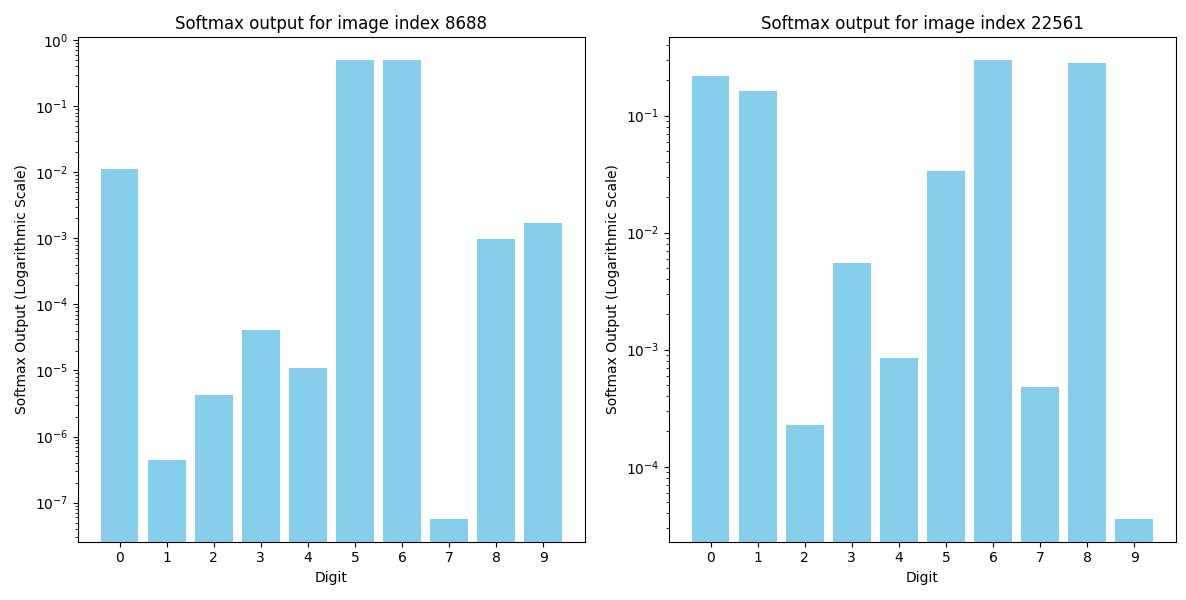
\includegraphics[width=0.99\columnwidth]{Figures/8688_22561_Softmax_Output.png}
    \caption{The Softmax output for the two "misclustered images in the correctly classified MNIST training dataset. Both are labelled as digit six. The example on the left is assigned to cluster 5 while the example on the right is assigned to cluster 8}
    \label{fig:8688_22561_Softmax_Output}
\end{figure}

Looking at the pattern of the softmax output (network prediction) 
indicates how confident a model is of the class prediction. Figure \ref{fig:8688_22561_Softmax_Output} contains two bar charts that show the MNIST-trained CNN softmax output for MNIST dataset digit ids 8688 and 22561 (starting from index 0), where both are labelled as class 6 and correctly classified by the CNN as such. The bar chart on the left shows the softmax output assigns a very high probability to both classes 5 and 6 (where 6 is the highest). The bar chart on the right shows that the CNN assigns a high probability to classes 6 and 8 (where 6 is again the highest). The cluster labels however do not correspond as digit id 8688 is nearer to the cluster 5 centroid, and digit id 22561 is nearer to cluster 8 centroid. This volatility may be explained by the relatively high deltas shown in Table \ref{tab:diff_softmax_avg_dist_to_centroids}, where the K-Means centroids moved a relatively large distance with respect to the initial values (given by average softmax outputs for correct digit classifications in the training dataset), for digit classes 5, 6 and 8. 

Conversely, the pattern of the distance to class centroids for a given softmax output 
indicates how close the softmax output is to a class centroid with respect to other class centroids. Figure \ref{fig:distances_to_centroids_8688_22561} shows on the left the distance to all class centroids of digit id 8688 network softmax output, placing it closing to centroids 5 and 6, while the image on the right (digit id 22561) places the softmax output closer to centroids 6 and 9. We notice the inverse relation between both sets of figures, where the highest bars (network confidence) in the first set correspond to the lowest bars (distance to class centroid) set in the second set.

% Clustering
% Repo: https://github.com/dsikar/work-in-progress.git
% retrieve data
% train_np = np.load('train_np.npy')
% train_np_with_indices = add_row_index(train_np)
% correct_preds = train_np_with_indices[train_np[:, 10] == train_np_with_indices[:, 11]]


% clustering_mismatches = find_clustering_mismatches(cluster_labels, correct_preds)

% Code to retrieve image
% Repo: https://github.com/dsikar/pmnist.git
% filename = '/home/daniel/git/work-in-progress/scripts/data/MNIST/raw/train-images-idx3-ubyte'
% index = 8688
% display_mnist_img(filename, index, verbose = False) 
% index = 22561
% display_mnist_img(filename, index, verbose = False)
\begin{figure}[H]
    \centering
    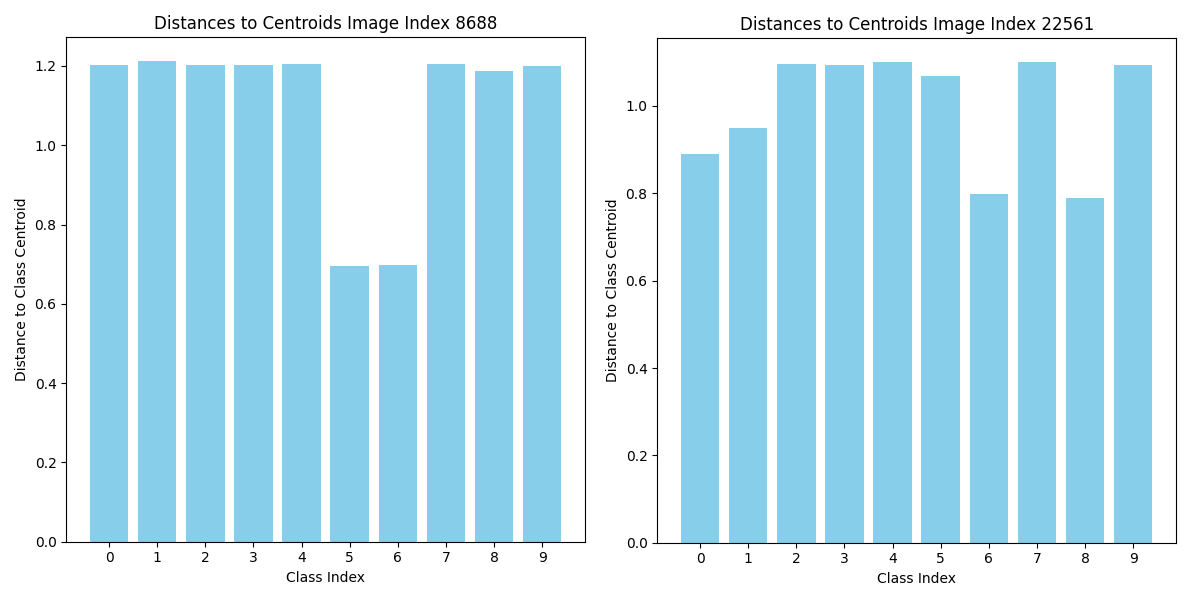
\includegraphics[width=0.99\columnwidth]{Figures/distances_to_centroids_8688_22561.png}
    \caption{The Softmax prediction distance to centroids for MNIST training images indexes 8688 (left) and 22561 (right), where both images are digit class 6, and the left image is misclassified as digit class 5, while the right image is misclassified as digit class 8.}
    \label{fig:distances_to_centroids_8688_22561} 
\end{figure}


% Code:
% import matplotlib.pyplot as plt
% import seaborn as sns

% plt.figure(figsize=(8, 6))
% sns.heatmap(likelihood_matrix, annot=True, cmap="YlGnBu", square=True, 
%             cbar_kws={"label": "Misclassification Likelihood"},
%             annot_kws={"size": 8}) 
% plt.xlabel("Misclassified Class")
% plt.ylabel("True Class")
% plt.title("Digit Class Misclassification Likelihood Matrix")
% plt.show()

% import pandas as pd

% likelihood_df = pd.DataFrame(likelihood_matrix, index=range(num_classes), columns=range(num_classes))
% print("Digit Class Misclassification Likelihood Matrix:")
% print(likelihood_df)

%%%%%%%%%%%%%%%%%%%%%%%%%%
% APPLYING PERTURBATIONS %
%%%%%%%%%%%%%%%%%%%%%%%%%%

\subsection{Applying Perturbations}
Through trial and error, we find sets of parameter values
for each perturbation function, such that as the level increases from 1 to
10, the network predictive accuracy decreases from 98.52\%
maximum to 36.32\% minimum and from average 97.61\%
(level 1) to 48.83\% (level 10). The accuracy degradation can be observed both Figures 
\ref{fig:Accuracy_vs_Noise_types} and \ref{fig:Pixelation_Digit_5_images_histogramsx10_plus_softmax}.

\begin{figure}[h] 
\begin{center}
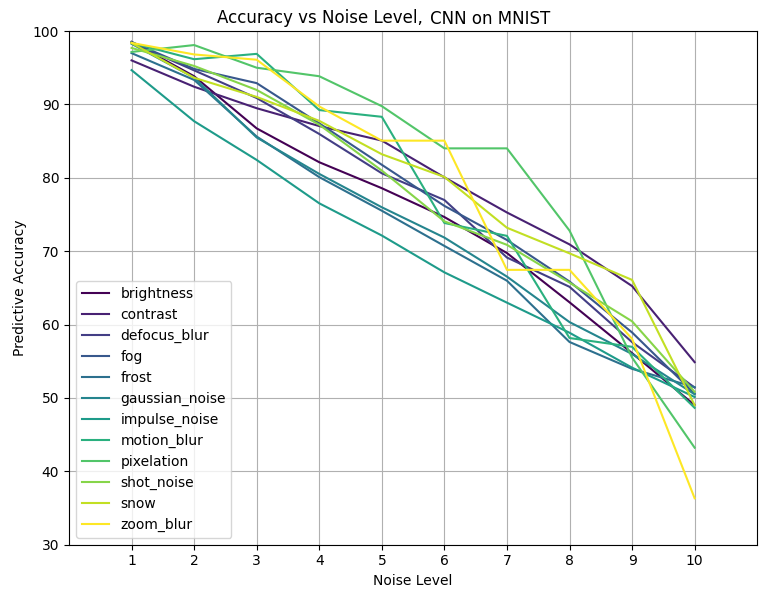
\includegraphics[width=0.99\columnwidth]{Figures/accuracy_vs_noise_types_plot.png}
\end{center}
\caption{Plot for network accuracy degradation for individual perturbation types: Brightness, Contrast, Defocus Blur, Fog, Frost, Gaussian Noise, Impulse Noise, Motion Blur, Pixelation, Shot Noise, Snow and Zoom Blur.}
\label{fig:Accuracy_vs_Noise_types}
\end{figure}

Figure \ref{fig:Pixelation_Digit_5_images_histogramsx10_plus_softmax} shows digit class 5 subject to increasing levels of pixelation from left to right. The bottom row of the figure shows the average softmax output for all perturbation types at a given level. We note that at all levels from 1 to 10, the highest prediction is digit class 5 (sixth column from left to right on every plot, the first being for digit 0).
\begin{figure*}[h!]
    \centering
    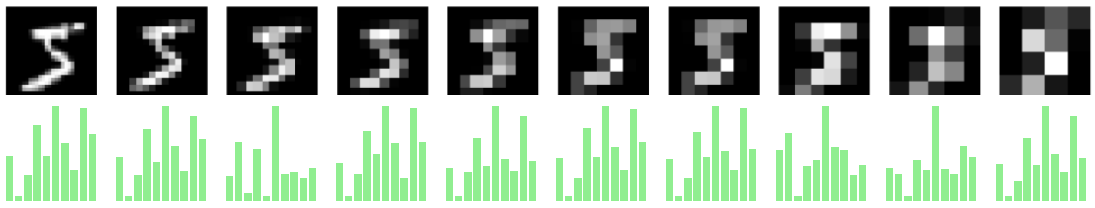
\includegraphics[width=0.99\textwidth]{Figures/Pixelation_Digit_5_images_histogramsx10_plus_softmax.png}   %\captionsetup{justification=raggedright,singlelinecheck=false}
    \caption{Top row: MNIST class digit 5 subject 1 to 10 levels of pixelation going left to right. Bottom row: the average softmax output for the perturbed MNIST dataset class digit 5 for each perturbation level across all perturbation types. The change in bar heights is an indication of how images are moving closer and further to centroids in the cluster as noise increases.}\label{fig:Pixelation_Digit_5_images_histogramsx10_plus_softmax}
\end{figure*}



% generated with function call visualize_accuracy_heatmap(accuracy_matrix, perturbation_types, intensities)
\begin{figure*}[h!]
    \centering
    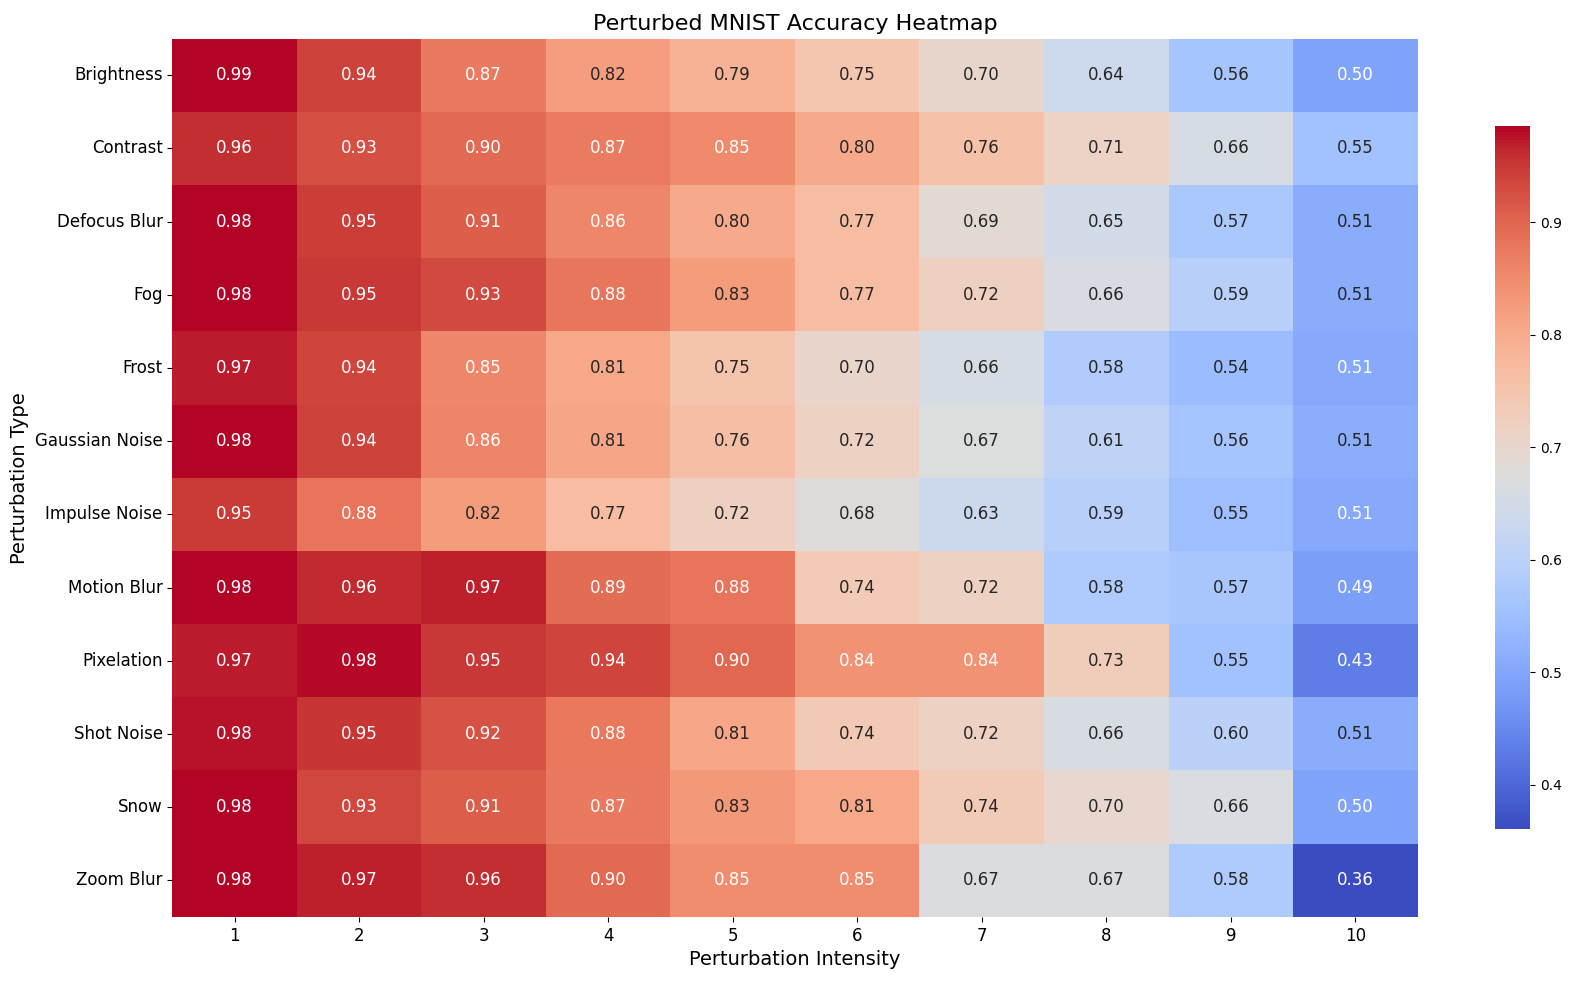
\includegraphics[width=0.99\textwidth]{Figures/PerturbedMNISTAccuracyHeatmap.png}   %\captionsetup{justification=raggedright,singlelinecheck=false}
    \caption{Perturbed MNIST Accuracy Heatmap, where the accuracies are for all digit classes, given a perturbation type and intensity.}
    \label{fig:PerturbedMNISTAccuracyHeatmap}
\end{figure*}

Figure \ref{fig:PerturbedMNISTAccuracyHeatmap} shows a heatmap where every cell represents one perturbation (y axis labels, 12 in total) at one intensity level (x axis labels, 10 in total) applied to the 10,000 image MNIST training dataset, the perturbed images are presented to the trained model and the resulting accuracy is placed in the corresponding cell. The heatmap therefore represents an experiment with 1,210,000 predictions on perturbed images of the perturbed dataset as described in section \ref{methods:PerturbedMNISTDataset}.

The heatmap uses a color scale from red to blue, with red indicating higher accuracy values and blue representing lower accuracy. As the perturbation intensity increases, the accuracy decreases for all perturbation types.

Some perturbations, such as brightness, contrast, and defocus blur, have a more gradual impact on accuracy as the intensity increases. For example, the accuracy under brightness perturbation drops from 0.99 at intensity 1 to 0.50 at intensity 10. Other perturbations, like pixelation and zoom blur, cause a more rapid decrease in accuracy at higher intensities.

Interestingly, certain perturbations, such as snow and impulse noise, show a slight increase in accuracy at lower intensities (e.g., intensity 2) compared to the baseline (intensity 1). This suggests that a small amount of these perturbations might act as a form of data augmentation, potentially improving the model's robustness.

The model appears to be most resilient to perturbations like brightness, contrast, and fog, maintaining relatively high accuracy even at higher intensities. On the other hand, perturbations such as pixelation, shot noise, and zoom blur have a more substantial negative impact on accuracy, with values dropping below 0.6 at higher intensities.

%%%%%%%%%%%%%%%%%%%%%%%%%%%%%%%%%%%%%%%
% MISCLASSIFICATION LIKELIHOOD MATRIX %
%%%%%%%%%%%%%%%%%%%%%%%%%%%%%%%%%%%%%%%

\subsection{Misclassification Likelihood Matrix}

Figure \ref{fig:DigitClassMisclassificationLikelihoodMatrix} shows the Misclassification Likelihood Matrix obtained by the method described in section \ref{miss_class_matrix}. Comparing the figure with the MNIST testing (non-perturbed) dataset shown in Figure \ref{fig:mnist_testing_dataset_confusion_matrix} we can notice some information added by the MLM that may help inform risk assessment. On the top right of the confusion matrix is a cluster of zeros, representing digits 0, 1 and 2 misclassifications of 8 and 9. The MLM is able to provide fine-grained information about the misclassification likelihood, assigning relatively low albeit non-zero likelihood misclassification values.
As the MLM represents a much larger dataset, there are some noticeable discrepancies. The MLM does not assign a high likelihood for digit 9 misclassified as 7, which is the highest in the testing dataset. On the other hand, row 7 is a close match with 7 being misclassified as 2 holding in the perturbed MNIST dataset.

MLM and traditional confusion matrices offer complementary insights into a neural network's classification performance. The MLM, derived from multiple perturbed versions of the testing set, provides a fine-grained view of misclassification tendencies. It represents the likelihood of each digit class being misclassified as another, with color intensity indicating misclassification probability. In contrast, the confusion matrix shows actual counts of correct and incorrect classifications for a single test set.
The MLM offers an additional perspective, showing likelihood values even for rare misclassifications.

While the confusion matrix clearly shows classification performance with higher numbers on the diagonal indicating better accuracy, the MLM requires a different interpretation. Zero values on the diagonal mean one class cannot be misclassified as itself. Both tools highlight patterns like the high likelihood of misclassifying 7 as 2, while the MLM also shows likelihood for corresponding zero values in the confusion matrix e.g. the likelihood of class zero being misclassified as classes 1, 2, 3, 4 or 5.

% Code:
% # Generate Distance Matrix
% num_classes = 10
% distance_matrix = generate_distance_matrix(test_np_with_distances, centroids, num_classes)
% import matplotlib.pyplot as plt
% import seaborn as sns

% plt.figure(figsize=(8, 6))
% sns.heatmap(distance_matrix, annot=True, cmap="YlGnBu", square=True, cbar_kws={"label": "Nearest Distance"}, annot_kws={"size": 8})
% plt.xlabel("Misclassified Class")
% plt.ylabel("True Class")
% plt.title("Nearest Distances To Other Digit Class Centroids")
% plt.show()
% \begin{figure}[h!]
%     \centering
%     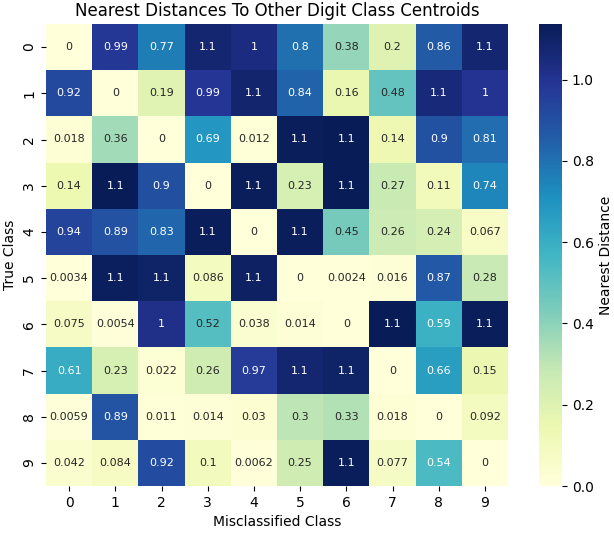
\includegraphics[width=0.99\columnwidth]{Figures/NearestDistancesToOtherDigitClassCentroids.png}
%     \caption{NearestDistancesToOtherDigitClassCentroids.}
%     \label{fig:NearestDistancesBetweenDigitClasses}
% \end{figure}

